\documentclass[a4paper,landscape]{article}
\usepackage{tikz}
\usepackage{gensymb}
\usepackage[utf8]{inputenc}
\usepackage[left=1cm,top=1cm,right=1cm,bottom=1cm,verbose,nohead,nofoot]{geometry}
\begin{document}
\pagenumbering{gobble}
\thispagestyle{empty}
\begin{center} 
\large\textbf{1\degree Andar}\\
\vspace*{5px} 
\large
\textmd{Comprimento: 29  -  Profundidade: 21  -  Altura: 25 (cm)}\\ \end{center}
\centering
\resizebox{!}{0.9\textheight}{%
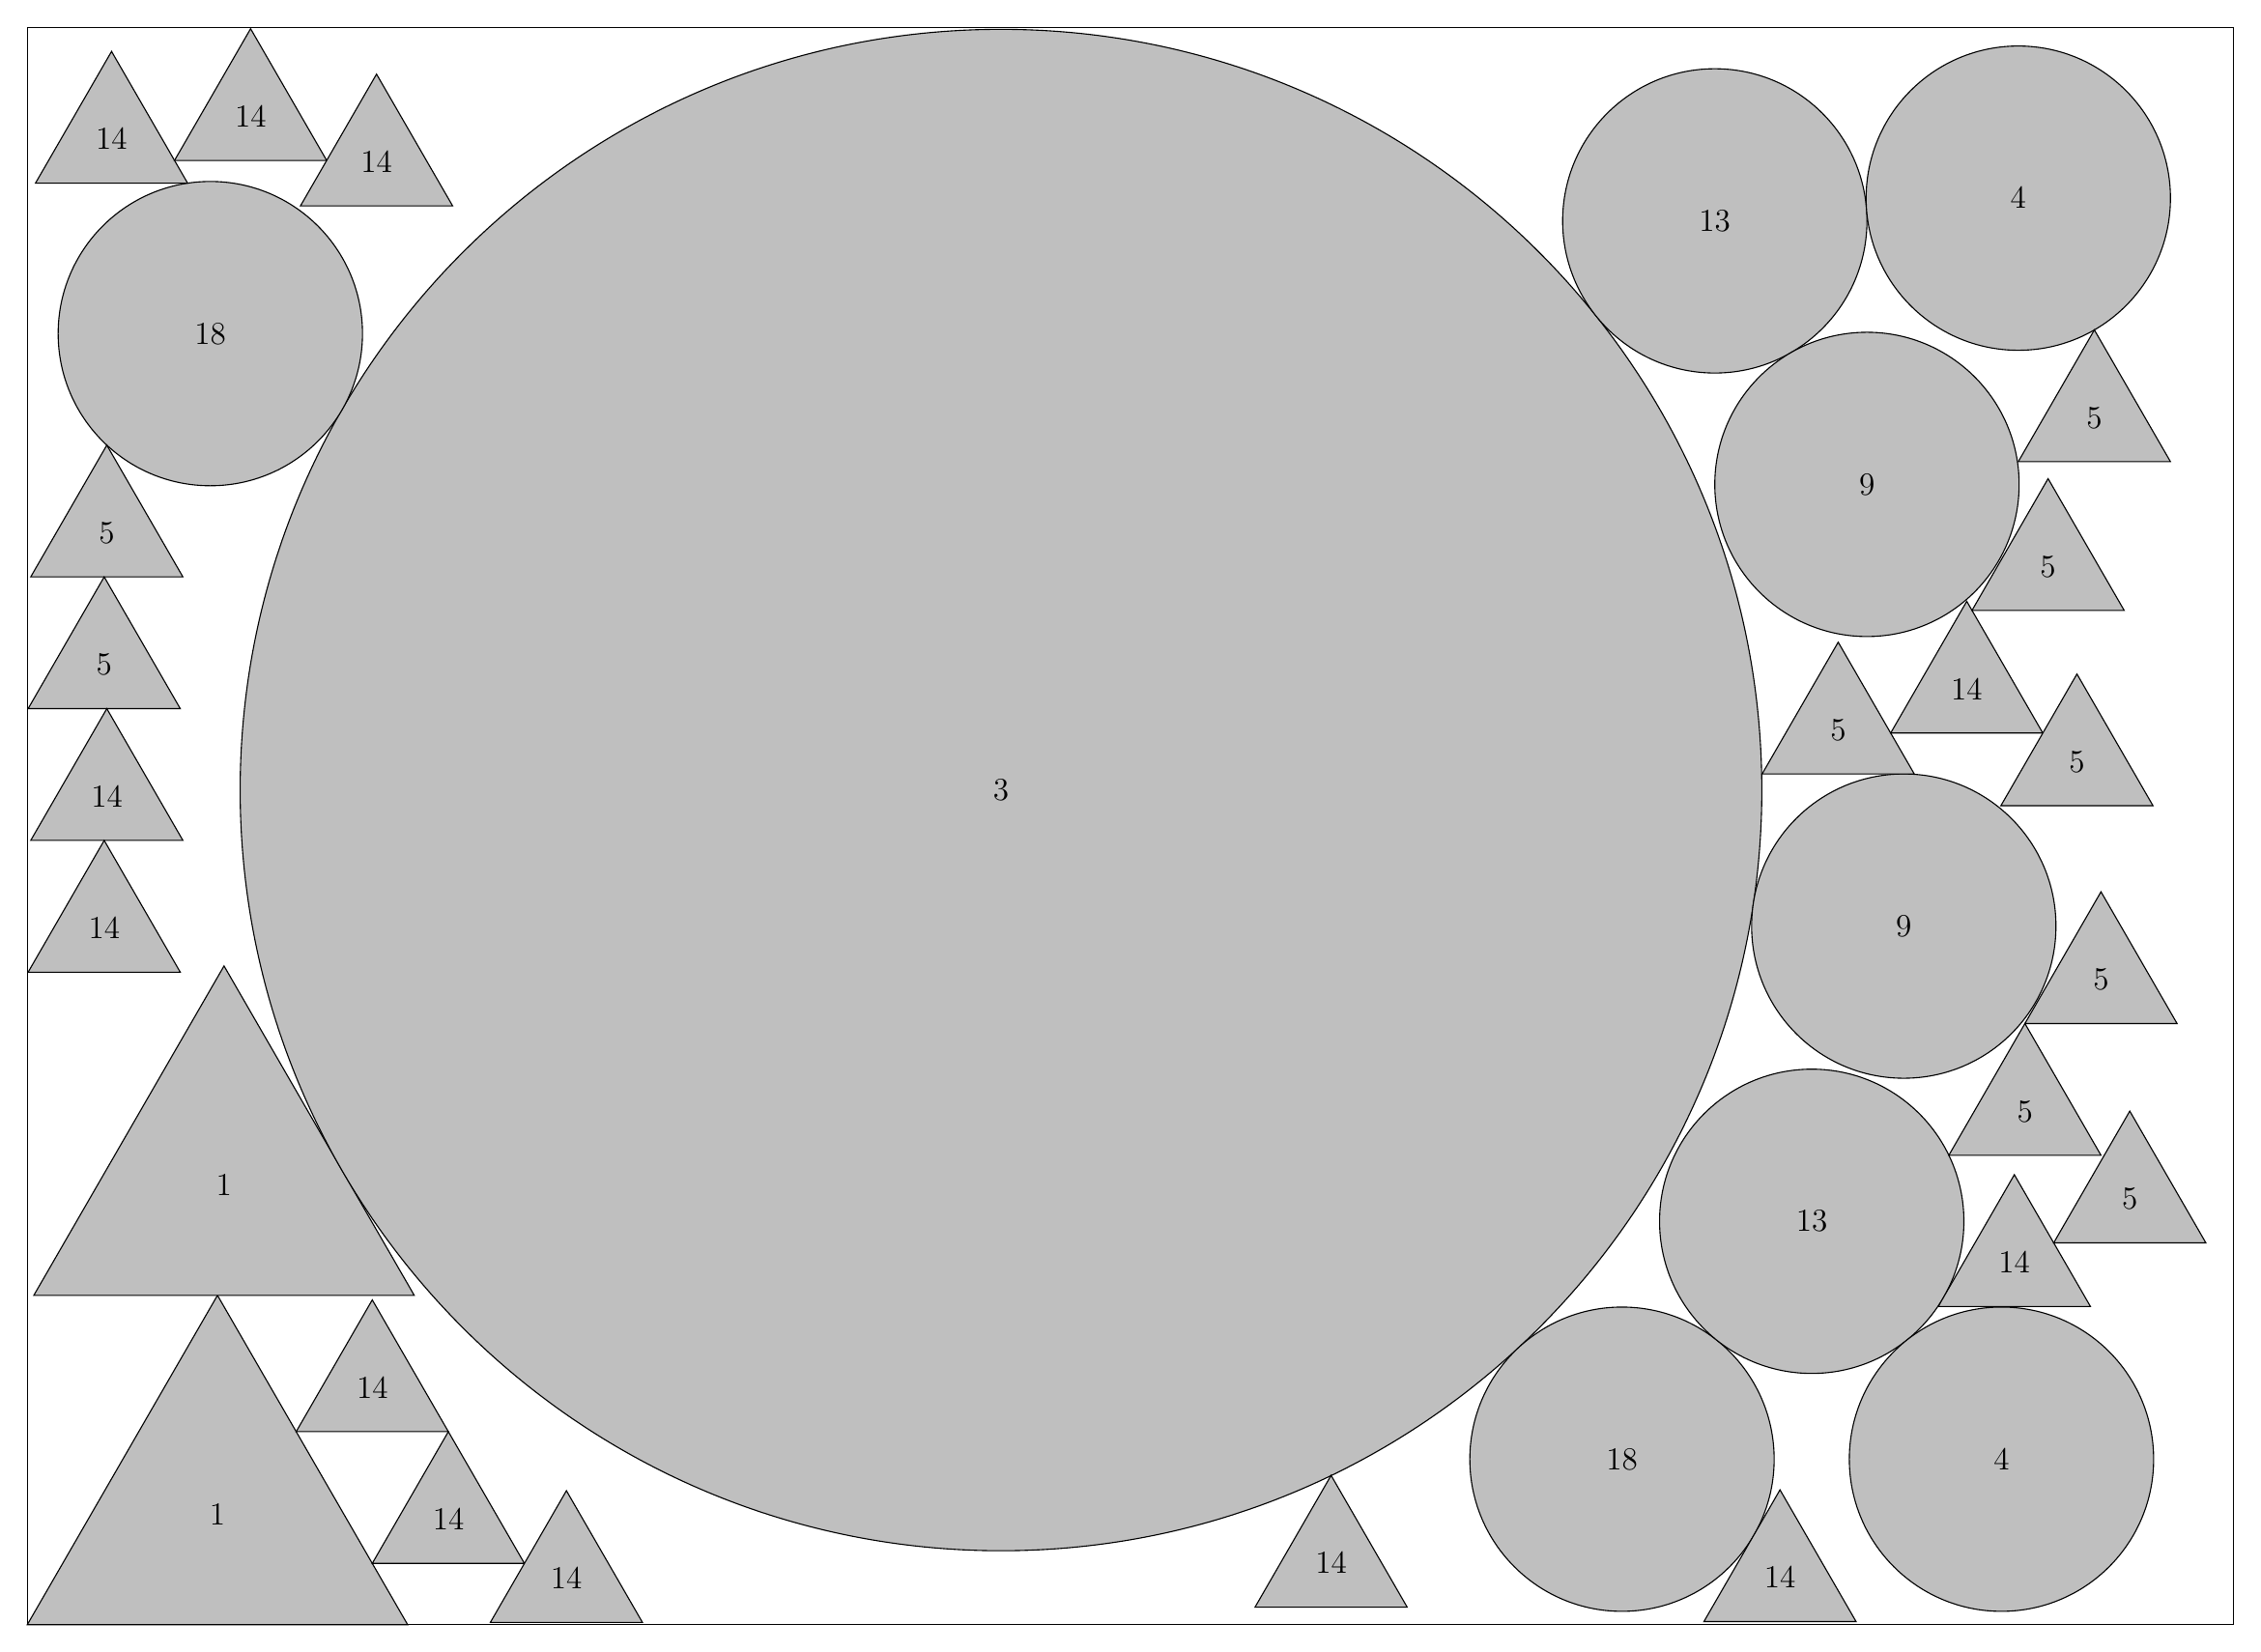
\begin{tikzpicture}\draw[black] (0,0) rectangle (29, 21);
\draw[black, fill=lightgray] (0,0) -- (5, 0) -- (2.5, 4.33013) -- cycle;
\draw (2.5, 1.44338) node {\large 1};
\draw[black, fill=lightgray] (0.0862069,4.33013) -- (5.08621, 4.33013) -- (2.58621, 8.66025) -- cycle;
\draw (2.58621, 5.7735) node {\large 1};
\draw[black, fill=lightgray] (12.7982,10.9726) circle (10);
\draw (12.7982, 10.9726) node {\large 3};
\draw[black, fill=lightgray] (2.40588,16.9726) circle (2);
\draw (2.40588, 16.9726) node {\large 18};
\draw[black, fill=lightgray] (20.9603,2.17597) circle (2);
\draw (20.9603, 2.17597) node {\large 18};
\draw[black, fill=lightgray] (22.1802,18.4545) circle (2);
\draw (22.1802, 18.4545) node {\large 13};
\draw[black, fill=lightgray] (23.4542,5.30329) circle (2);
\draw (23.4542, 5.30329) node {\large 13};
\draw[black, fill=lightgray] (24.1802,14.9904) circle (2);
\draw (24.1802, 14.9904) node {\large 9};
\draw[black, fill=lightgray] (24.6642,9.18408) circle (2);
\draw (24.6642, 9.18408) node {\large 9};
\draw[black, fill=lightgray] (25.9482,2.17597) circle (2);
\draw (25.9482, 2.17597) node {\large 4};
\draw[black, fill=lightgray] (26.169,18.7534) circle (2);
\draw (26.169, 18.7534) node {\large 4};
\draw[black, fill=lightgray] (0.0455348,13.7744) -- (2.04553, 13.7744) -- (1.04553, 15.5065) -- cycle;
\draw (1.04553, 14.3518) node {\large 5};
\draw[black, fill=lightgray] (0.011052,12.0424) -- (2.01105, 12.0424) -- (1.01105, 13.7744) -- cycle;
\draw (1.01105, 12.6197) node {\large 5};
\draw[black, fill=lightgray] (0.0455348,10.3103) -- (2.04553, 10.3103) -- (1.04553, 12.0424) -- cycle;
\draw (1.04553, 10.8877) node {\large 14};
\draw[black, fill=lightgray] (0.011052,8.57828) -- (2.01105, 8.57828) -- (1.01105, 10.3103) -- cycle;
\draw (1.01105, 9.15563) node {\large 14};
\draw[black, fill=lightgray] (0.107796,18.9503) -- (2.1078, 18.9503) -- (1.1078, 20.6823) -- cycle;
\draw (1.1078, 19.5276) node {\large 14};
\draw[black, fill=lightgray] (1.93538,19.2489) -- (3.93538, 19.2489) -- (2.93538, 20.9809) -- cycle;
\draw (2.93538, 19.8262) node {\large 14};
\draw[black, fill=lightgray] (3.53448,2.53835) -- (5.53448, 2.53835) -- (4.53448, 4.2704) -- cycle;
\draw (4.53448, 3.1157) node {\large 14};
\draw[black, fill=lightgray] (3.59055,18.6516) -- (5.59055, 18.6516) -- (4.59055, 20.3837) -- cycle;
\draw (4.59055, 19.229) node {\large 14};
\draw[black, fill=lightgray] (4.53448,0.8063) -- (6.53448, 0.8063) -- (5.53448, 2.53835) -- cycle;
\draw (5.53448, 1.38365) node {\large 14};
\draw[black, fill=lightgray] (6.08621,0.0298629) -- (8.08621, 0.0298629) -- (7.08621, 1.76191) -- cycle;
\draw (7.08621, 0.607213) node {\large 14};
\draw[black, fill=lightgray] (16.137,0.23085) -- (18.137, 0.23085) -- (17.137, 1.9629) -- cycle;
\draw (17.137, 0.8082) node {\large 14};
\draw[black, fill=lightgray] (22.0371,0.0411746) -- (24.0371, 0.0411746) -- (23.0371, 1.77323) -- cycle;
\draw (23.0371, 0.618525) node {\large 14};
\draw[black, fill=lightgray] (22.8021,11.1841) -- (24.8021, 11.1841) -- (23.8021, 12.9161) -- cycle;
\draw (23.8021, 11.7614) node {\large 5};
\draw[black, fill=lightgray] (24.4917,11.7216) -- (26.4917, 11.7216) -- (25.4917, 13.4537) -- cycle;
\draw (25.4917, 12.299) node {\large 14};
\draw[black, fill=lightgray] (25.1173,4.18384) -- (27.1173, 4.18384) -- (26.1173, 5.91589) -- cycle;
\draw (26.1173, 4.76119) node {\large 14};
\draw[black, fill=lightgray] (25.2562,6.17106) -- (27.2562, 6.17106) -- (26.2562, 7.90311) -- cycle;
\draw (26.2562, 6.74841) node {\large 5};
\draw[black, fill=lightgray] (25.5607,13.3342) -- (27.5607, 13.3342) -- (26.5607, 15.0663) -- cycle;
\draw (26.5607, 13.9116) node {\large 5};
\draw[black, fill=lightgray] (25.94,10.766) -- (27.94, 10.766) -- (26.94, 12.4981) -- cycle;
\draw (26.94, 11.3434) node {\large 5};
\draw[black, fill=lightgray] (26.169,15.2893) -- (28.169, 15.2893) -- (27.169, 17.0213) -- cycle;
\draw (27.169, 15.8666) node {\large 5};
\draw[black, fill=lightgray] (26.2562,7.90311) -- (28.2562, 7.90311) -- (27.2562, 9.63516) -- cycle;
\draw (27.2562, 8.48046) node {\large 5};
\draw[black, fill=lightgray] (26.6345,5.02) -- (28.6345, 5.02) -- (27.6345, 6.75205) -- cycle;
\draw (27.6345, 5.59735) node {\large 5};\end{tikzpicture}
}%
\newpage\clearpage
\thispagestyle{empty}
\begin{center} 
\large\textbf{2\degree Andar}\\
\vspace*{5px} 
\large
\textmd{Comprimento: 29  -  Profundidade: 21  -  Altura: 5 (cm)}\\ \end{center}
\centering
\resizebox{!}{0.9\textheight}{%
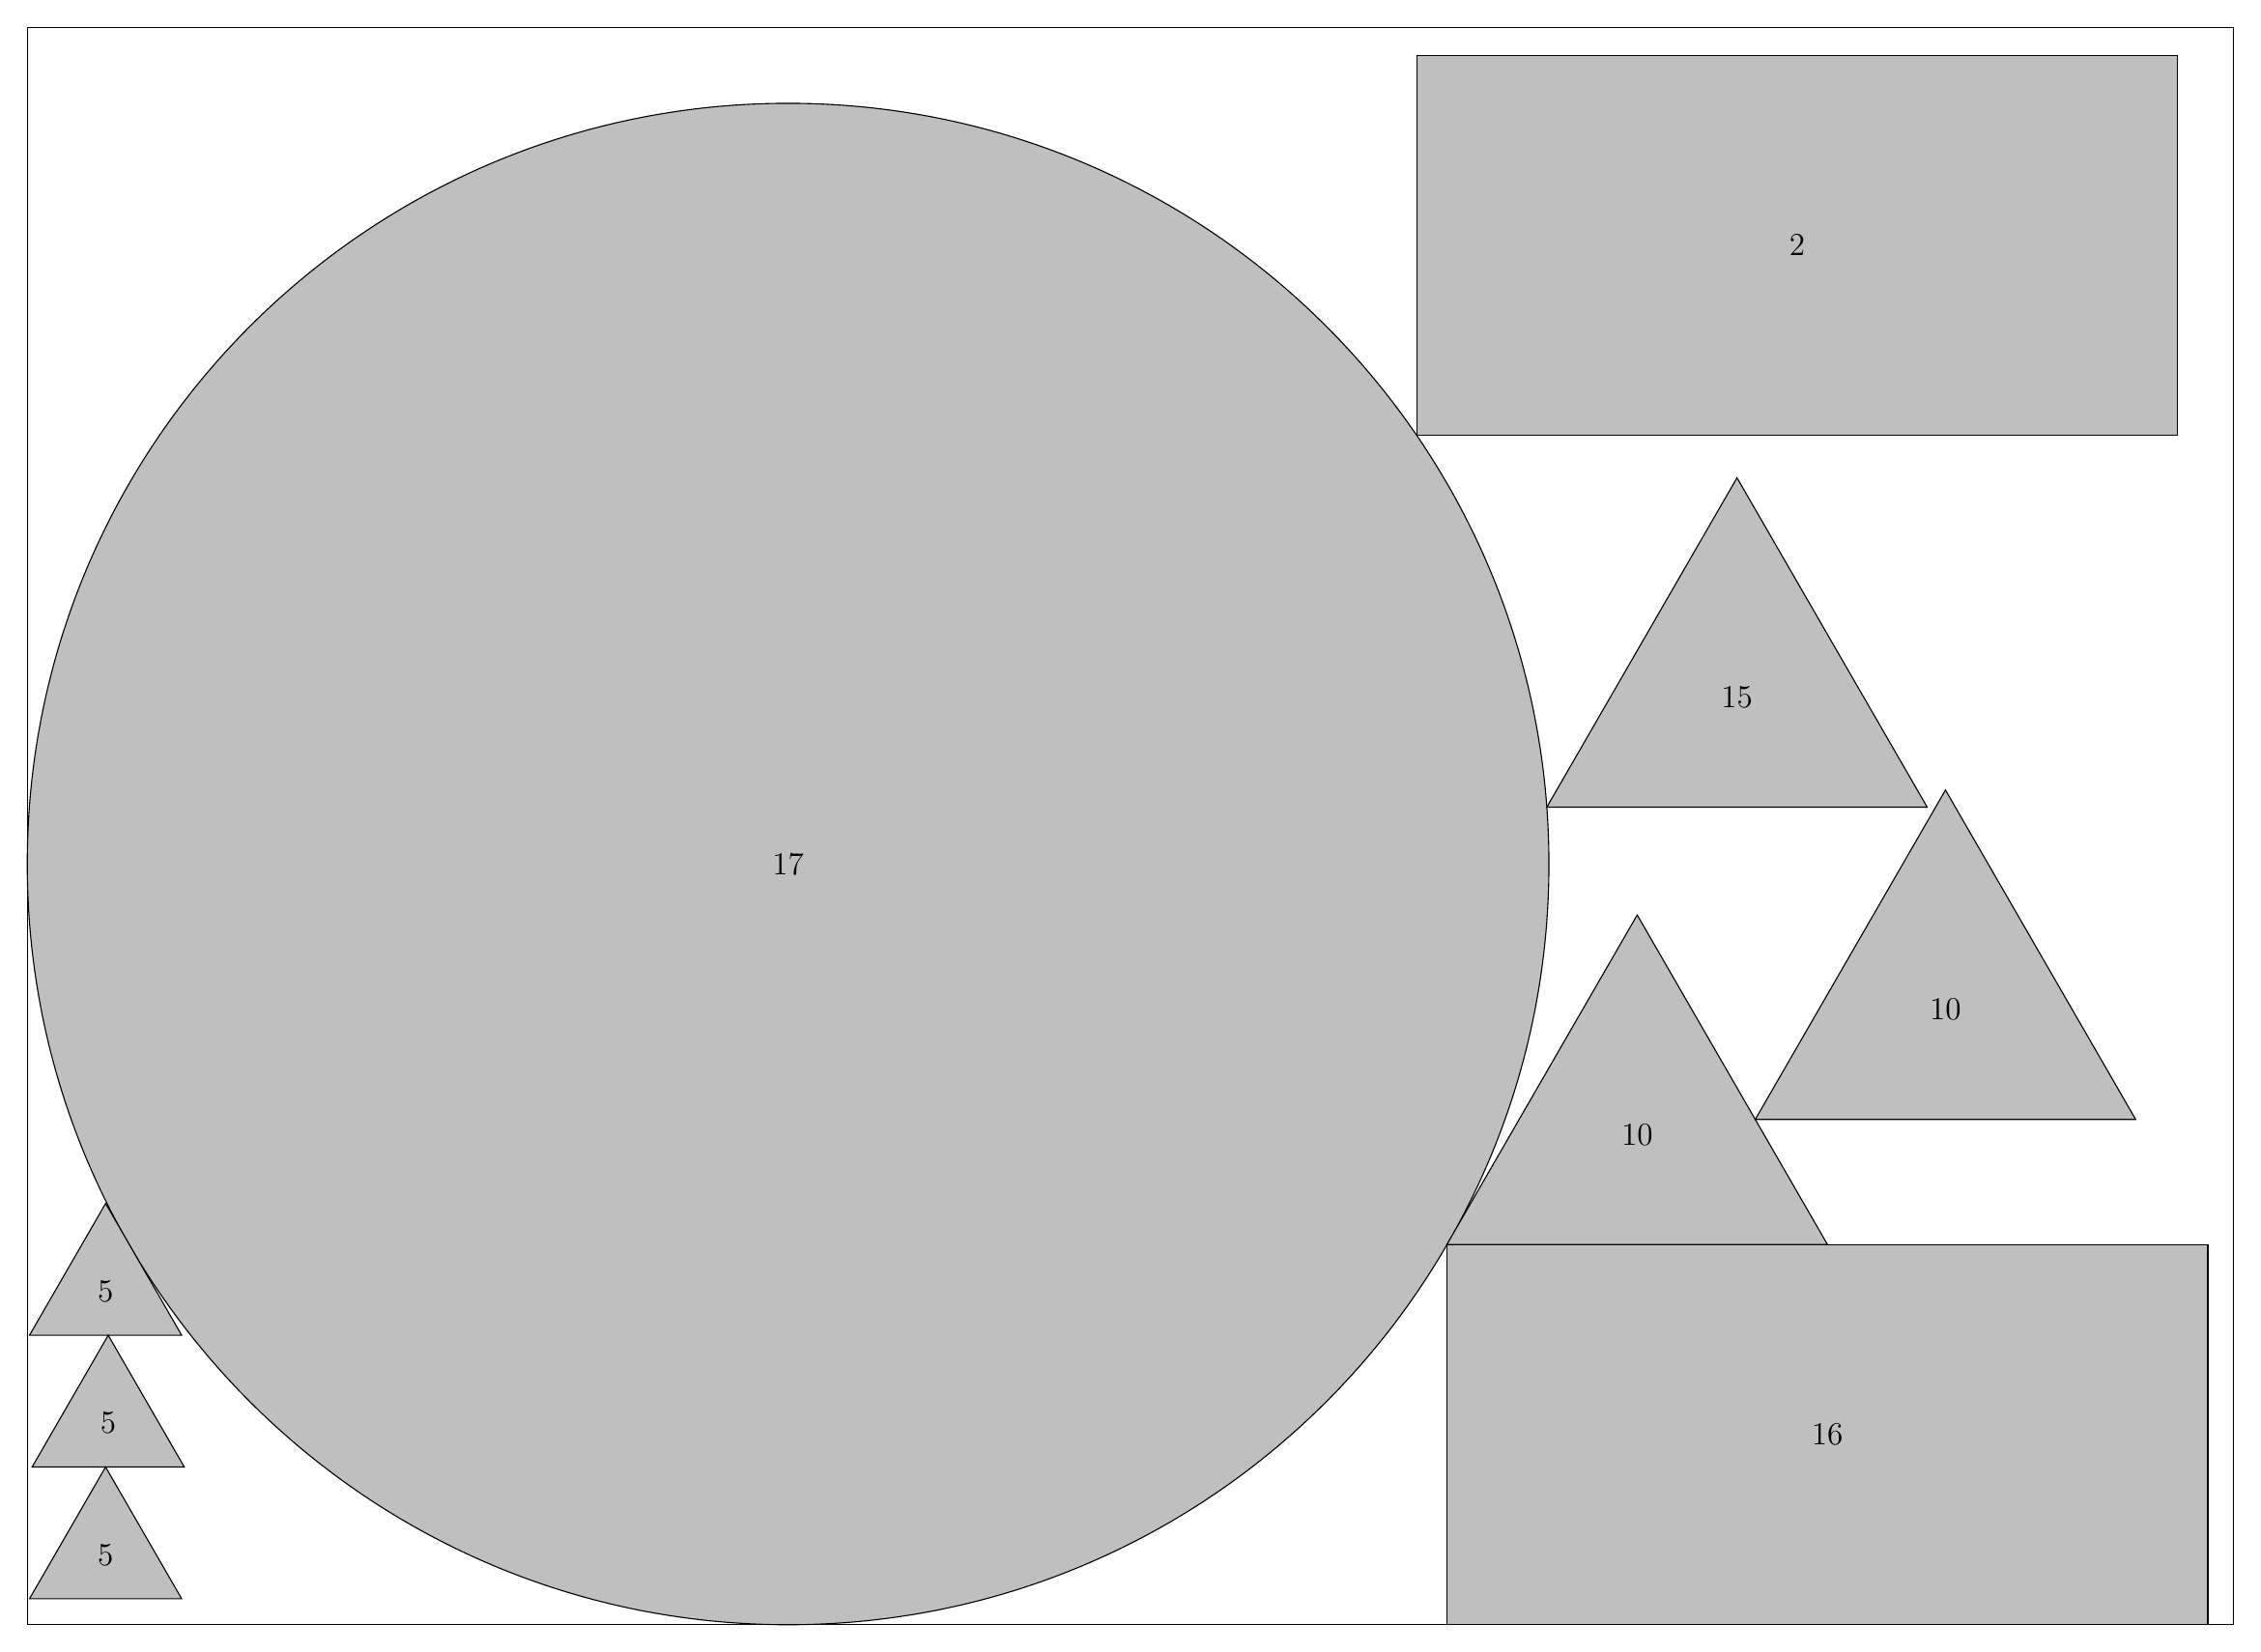
\begin{tikzpicture}\draw[black] (0,0) rectangle (29, 21);
\draw[black, fill=lightgray] (10,10) circle (10);
\draw (10, 10) node {\large 17};
\draw[black, fill=lightgray] (18.2624,15.6332) rectangle (28.2624, 20.6332);
\draw (23.2624, 18.1332) node {\large 2};
\draw[black, fill=lightgray] (18.6603,0) rectangle (28.6603, 5);
\draw (23.6603, 2.5) node {\large 16};
\draw[black, fill=lightgray] (18.6603,5) -- (23.6603, 5) -- (21.1603, 9.33013) -- cycle;
\draw (21.1603, 6.44338) node {\large 10};
\draw[black, fill=lightgray] (19.972,10.7473) -- (24.972, 10.7473) -- (22.472, 15.0774) -- cycle;
\draw (22.472, 12.1907) node {\large 15};
\draw[black, fill=lightgray] (22.712,6.64246) -- (27.712, 6.64246) -- (25.212, 10.9726) -- cycle;
\draw (25.212, 8.08584) node {\large 10};
\draw[black, fill=lightgray] (0.0294011,3.80548) -- (2.0294, 3.80548) -- (1.0294, 5.53753) -- cycle;
\draw (1.0294, 4.38283) node {\large 5};
\draw[black, fill=lightgray] (0.0638839,2.07343) -- (2.06388, 2.07343) -- (1.06388, 3.80548) -- cycle;
\draw (1.06388, 2.65078) node {\large 5};
\draw[black, fill=lightgray] (0.0294011,0.341381) -- (2.0294, 0.341381) -- (1.0294, 2.07343) -- cycle;
\draw (1.0294, 0.918731) node {\large 5};\end{tikzpicture}
}%
\newpage\clearpage
\thispagestyle{empty}
\begin{center} 
\large\textbf{3\degree Andar}\\
\vspace*{5px} 
\large
\textmd{Comprimento: 29  -  Profundidade: 21  -  Altura: 5 (cm)}\\ \end{center}
\centering
\resizebox{!}{0.9\textheight}{%
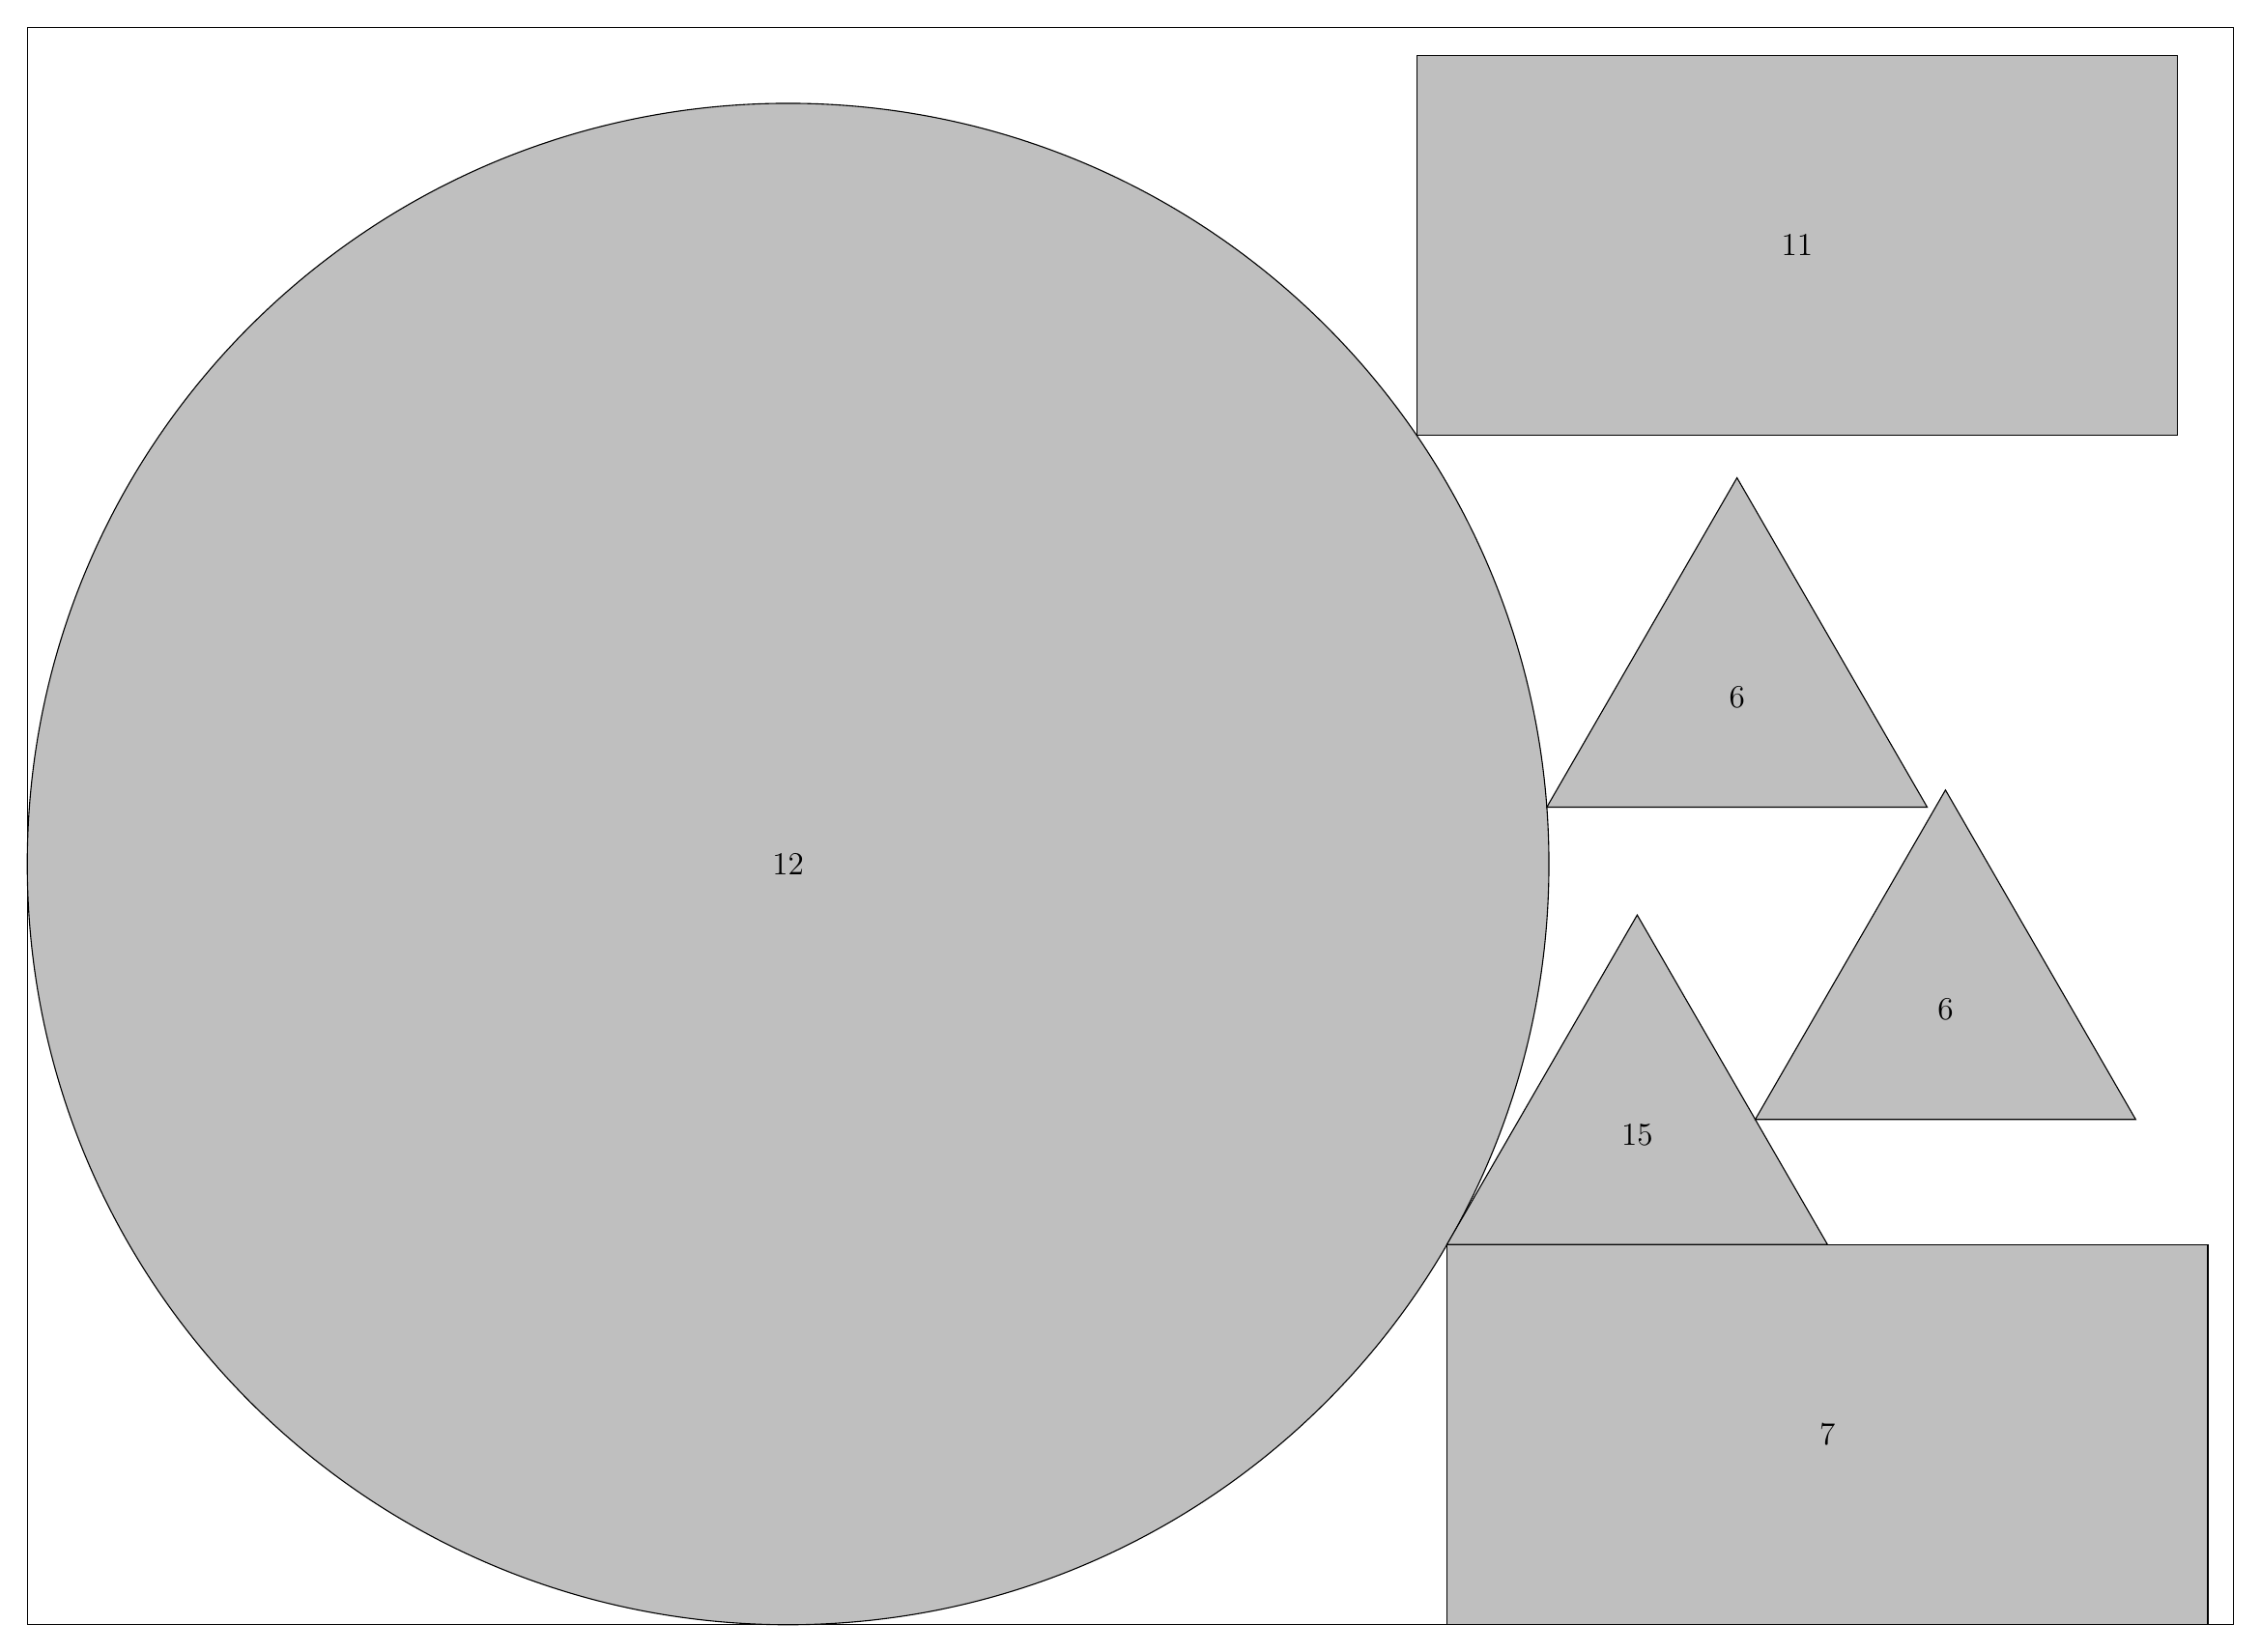
\begin{tikzpicture}\draw[black] (0,0) rectangle (29, 21);
\draw[black, fill=lightgray] (10,10) circle (10);
\draw (10, 10) node {\large 12};
\draw[black, fill=lightgray] (18.2624,15.6332) rectangle (28.2624, 20.6332);
\draw (23.2624, 18.1332) node {\large 11};
\draw[black, fill=lightgray] (18.6603,0) rectangle (28.6603, 5);
\draw (23.6603, 2.5) node {\large 7};
\draw[black, fill=lightgray] (18.6603,5) -- (23.6603, 5) -- (21.1603, 9.33013) -- cycle;
\draw (21.1603, 6.44338) node {\large 15};
\draw[black, fill=lightgray] (19.972,10.7473) -- (24.972, 10.7473) -- (22.472, 15.0774) -- cycle;
\draw (22.472, 12.1907) node {\large 6};
\draw[black, fill=lightgray] (22.712,6.64246) -- (27.712, 6.64246) -- (25.212, 10.9726) -- cycle;
\draw (25.212, 8.08584) node {\large 6};\end{tikzpicture}
}%
\newpage\clearpage
\thispagestyle{empty}
\begin{center} 
\large\textbf{4\degree Andar}\\
\vspace*{5px} 
\large
\textmd{Comprimento: 29  -  Profundidade: 21  -  Altura: 5 (cm)}\\ \end{center}
\centering
\resizebox{!}{0.9\textheight}{%
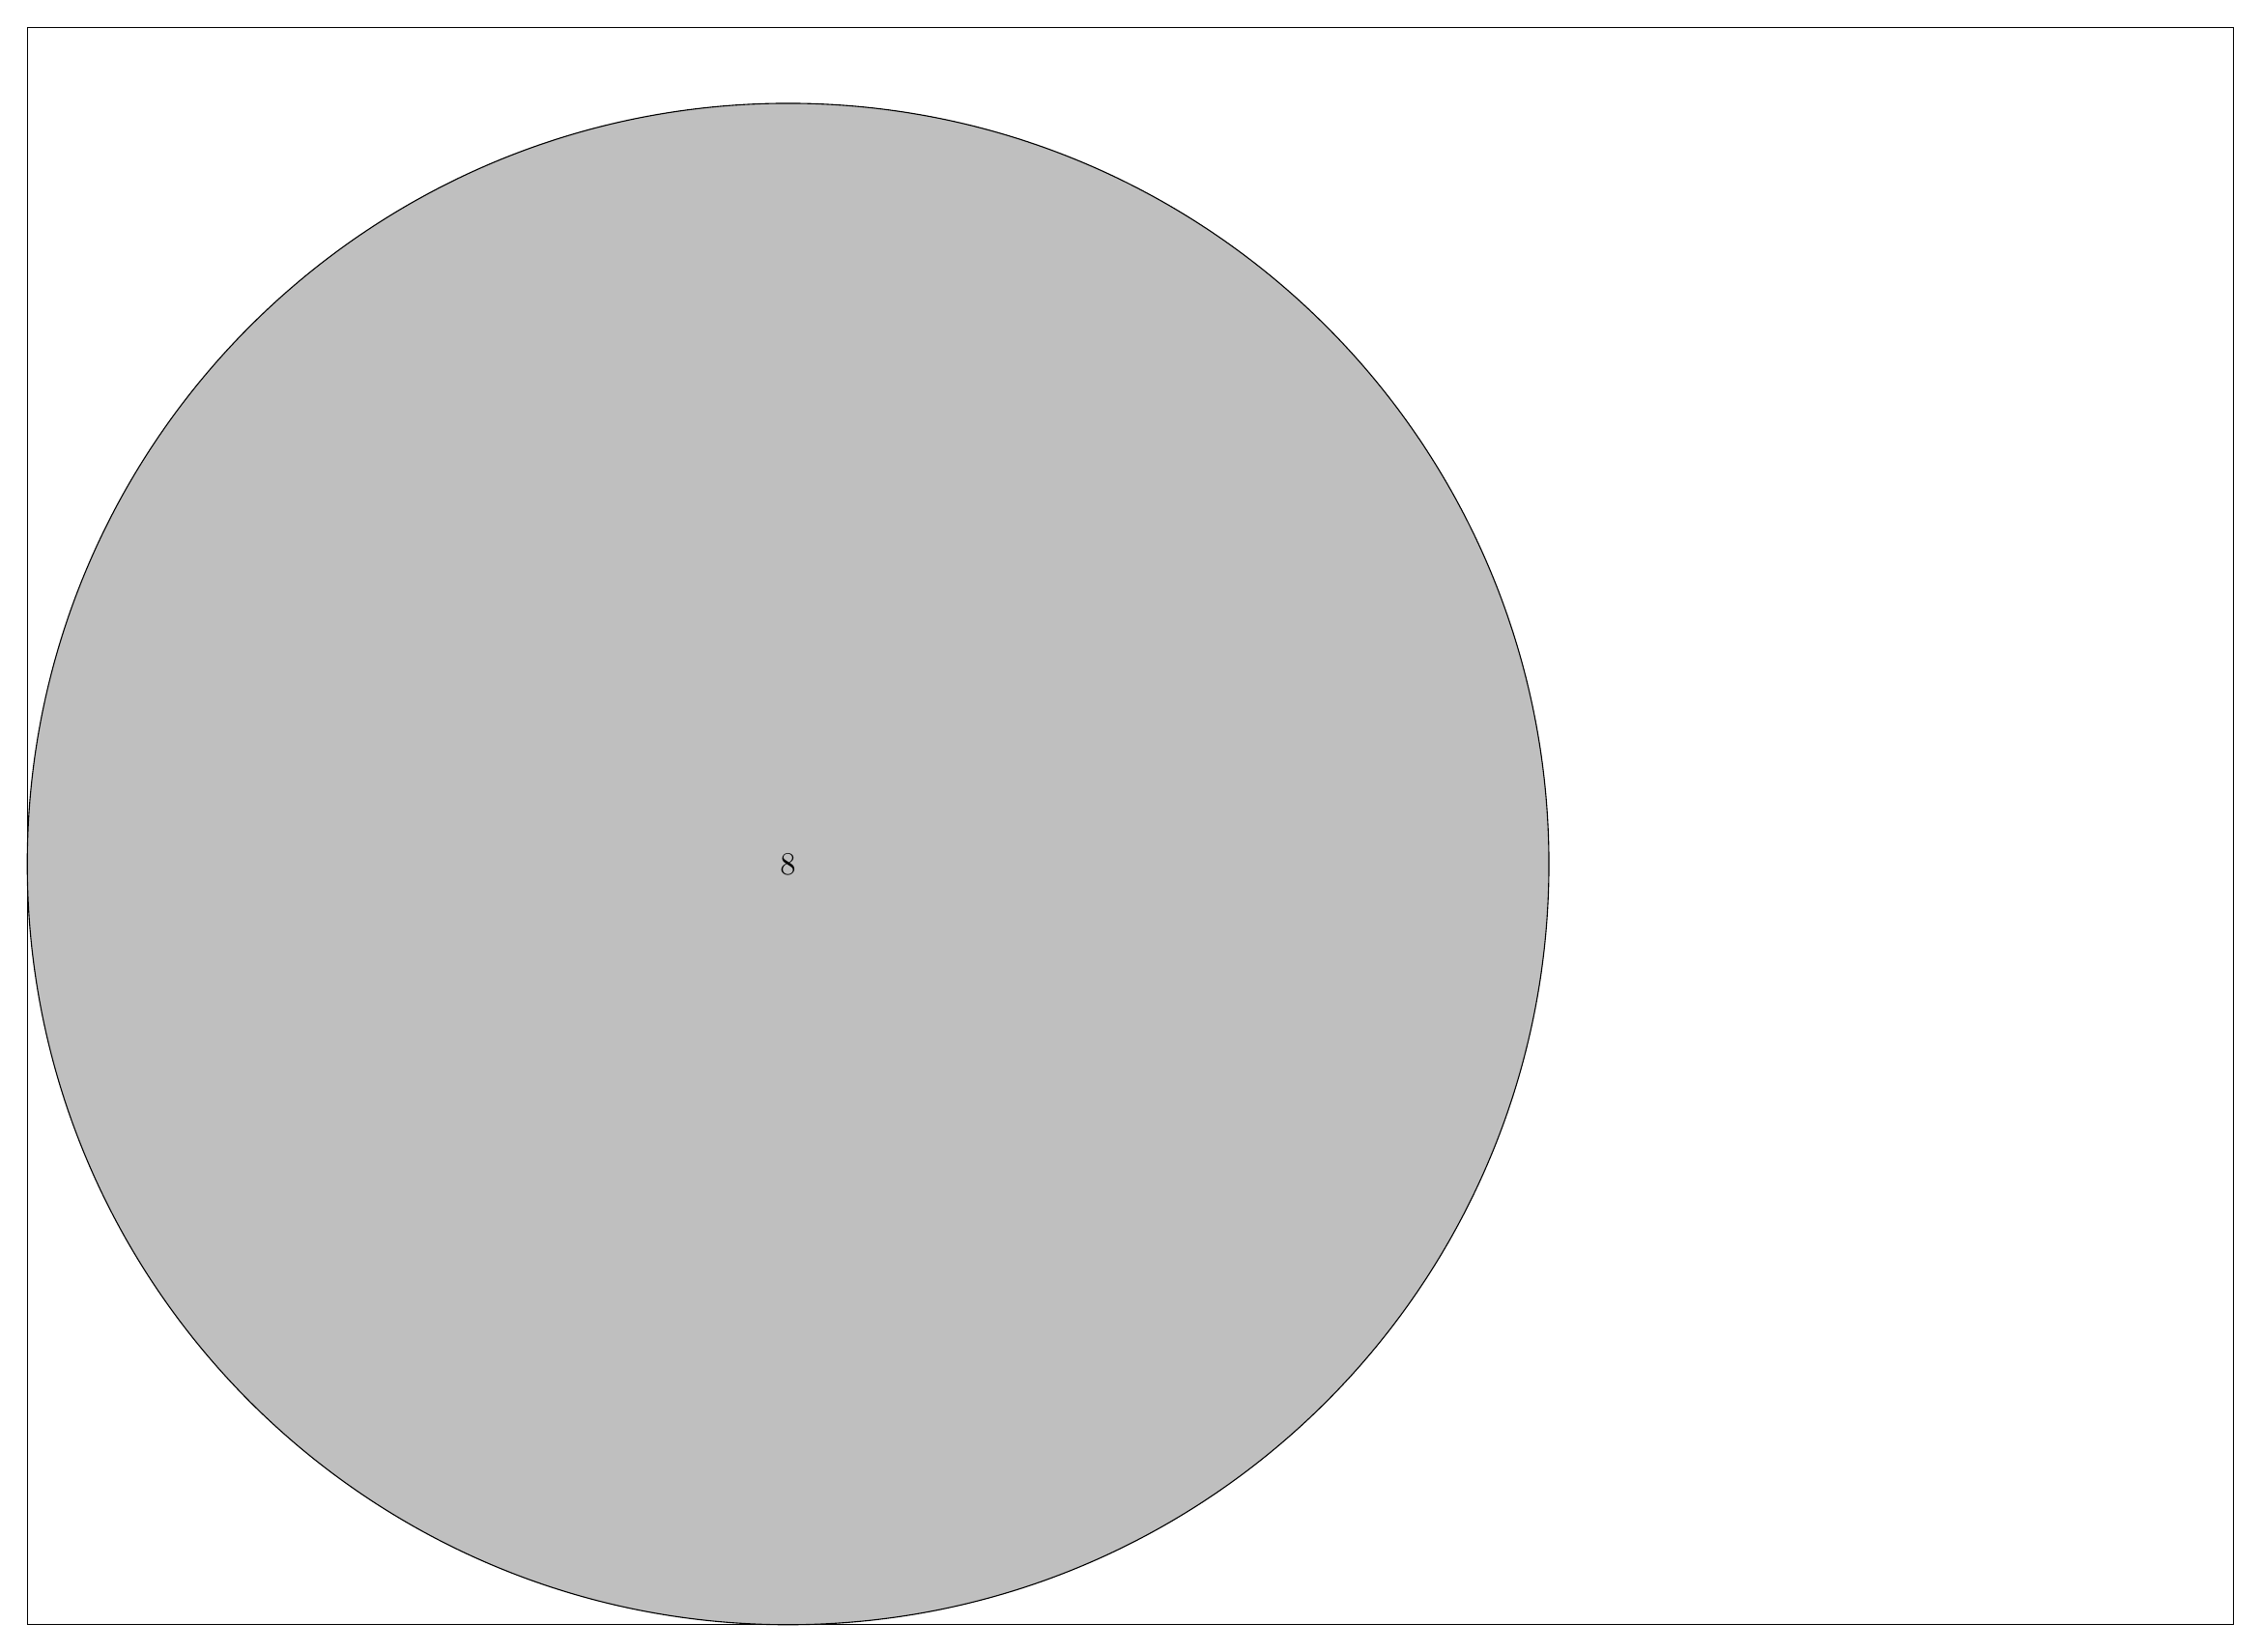
\begin{tikzpicture}\draw[black] (0,0) rectangle (29, 21);
\draw[black, fill=lightgray] (10,10) circle (10);
\draw (10, 10) node {\large 8};\end{tikzpicture}
}%
\newpage\clearpage\thispagestyle{empty}
\begin{center} 
\large
\textbf{Descrição das Peças}\\\vspace*{10px} 
 \end{center}\begin{enumerate}\item Description of triangle
\item Description of rectangle
\item Description of circle
\item Description of circle
\item triangle
\item Description of triangle
\item Description of rectangle
\item Description of circle
\item Description of circle
\item Description of triangle
\item Description of rectangle
\item Description of circle
\item Description of circle
\item triangle
\item Description of triangle
\item Description of rectangle
\item Description of circle
\item Description of circle
\end{enumerate}
\end{document}